\documentclass[]{article}
\usepackage{graphicx}
\usepackage{xcolor}
\usepackage{enumerate}
\usepackage{hyperref}
\hypersetup{%
  colorlinks = true,
  linkcolor  = black
}


% Title Page
\title{Software Engineering (CS301)\\ User Interface\\ Design (Version 1)\\Travel Diaries}
\author{Group 5}

\begin{document}
\maketitle


\begin{center}
\textbf{Project Members}\\
\vspace*{.6cm}
\begin{tabular}{|c|c|}
\hline
\textbf{ID} & \textbf{Name}\\
\hline
\hline
201452004 & Nilesh Chaturvedi\\
\hline
201452005 & Jitender Rajput\\
\hline
201452012 & Durga Vijaya Lakshmi\\
\hline
201452036 & Pedapalli Akhil\\
\hline
20152040 & B. Indu\\
\hline
201452044 & Dileep Krishna\\
\hline
201452050 & Shreya Singh\\
\hline
201452056 & Ravi Patel\\
\hline
201452057 & G. Raju Koushik\\
\hline
\end{tabular}

\vspace*{1cm}

\begin{tabular}{|c|c|}
\hline
\textbf{Authored By} & \textbf{Nilesh Chaturvedi, Jitendra Rajput}\\
\textbf{Reviewed By} & \textbf{B. Indu}\\
\hline
\end{tabular}
\end{center}

\newpage
\section{User Interface}
User interface design (UI) is the design of user interfaces for mobile software with the focus on maximizing the user satisfaction. The goal of
user interface design is to make the user’s interaction as simple and efficient as possible, in terms of accomplishing user goals (user-centered design). We have used proto.io to design UI for Android Mobile.

\subsection{Login Activity}
This the landing page for any user who installs the application for the first time in his/her mobile device. This lets the user to sign-in in his/her pre-existing account or sign-up if he/she is new to the application. Two optins are provided to the user for sign-up, i.e. manual sign-up and sign-in using google. If the user has a google account, then the same can be user for registration.\\ \\
\begin{center}
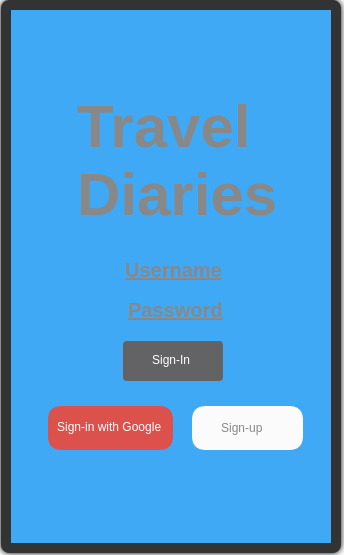
\includegraphics[scale=.45]{login.png}}  \\ 
\caption{Figure 1:  Login Page}
\end{center}
\newpage

\subsection{Register Activity}
This activity pops up when the user clicks on sign-up button. The user can fill-in his/her details and get registered on the application.
    
\begin{center}
\includegraphics[scale=.45]{Register.png}}\\
\caption{Figure 2:  Register Activity}
\end{center}

\newpage
\subsection{Home Activity}
This is the activity where the user lands once he has successfully signed in and subsequent access of the application. Here the items in the label list are the posts from various users. The user can add his/her post by clicking the` +` icon. The user can also search for diaries.
\begin{center}
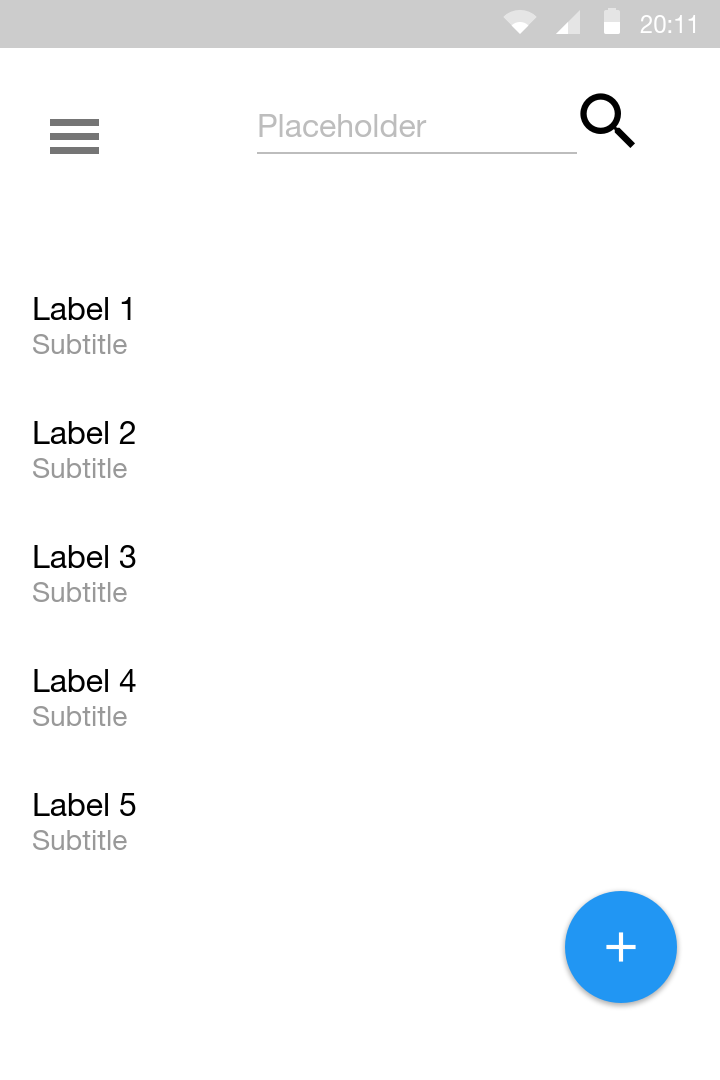
\includegraphics[scale=.40]{Home.png}}\\
\caption{Figure 3:  Home Activity}
\end{center}

\newpage


\subsection{Add Post}
This is the activity that the user makes use of while posting something on the application. Here the user can search or simply tap on the location icon if he wants to post about the current place. The user can enter a small description of the place in the given space.Furthermore the user can upload or capture a photograph of the place which would further be geo-tagged based on the location.
\begin{center}
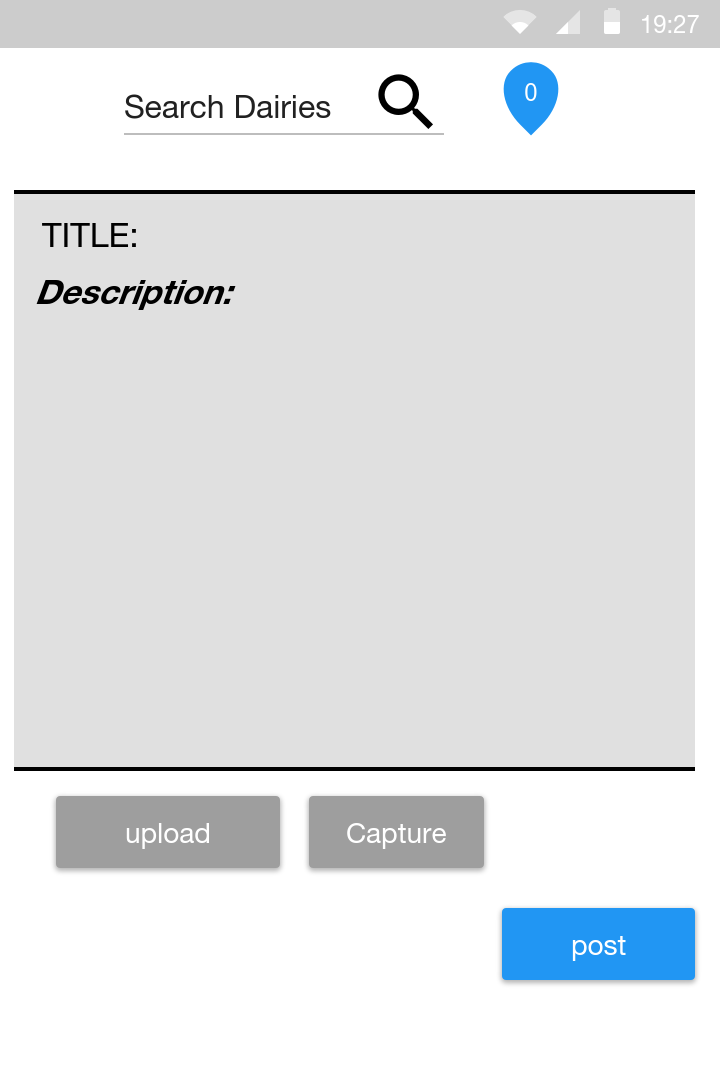
\includegraphics[scale=.40]{AddPost.png}}\\
\caption{Figure 4:  Add Post}
\end{center}

\newpage

\subsection{Search Diary}
Here the user can search for the various diaries and the posts associated with the diary. The user also has an option to follow that diary.
\begin{center}
\includegraphics[scale=.40]{SearchDiaries.png}}\\
\caption{Figure 5:  Search Diaries}
\end{center}

\newpage

\subsection{Follwers/Following}
Here the user can search for the various diaries and the posts associated with the diary. The user also has an option to follow that diary.
\begin{center}
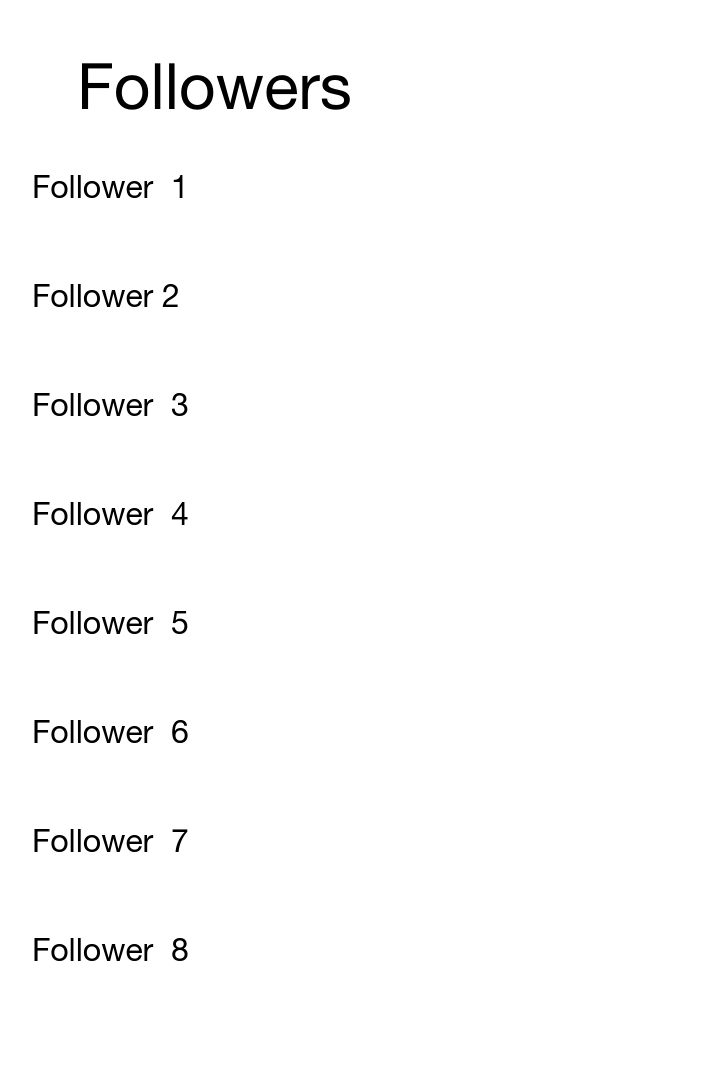
\includegraphics[scale=.20]{Followers.png}}\\
\caption{Figure 6.1:  Followers}\\
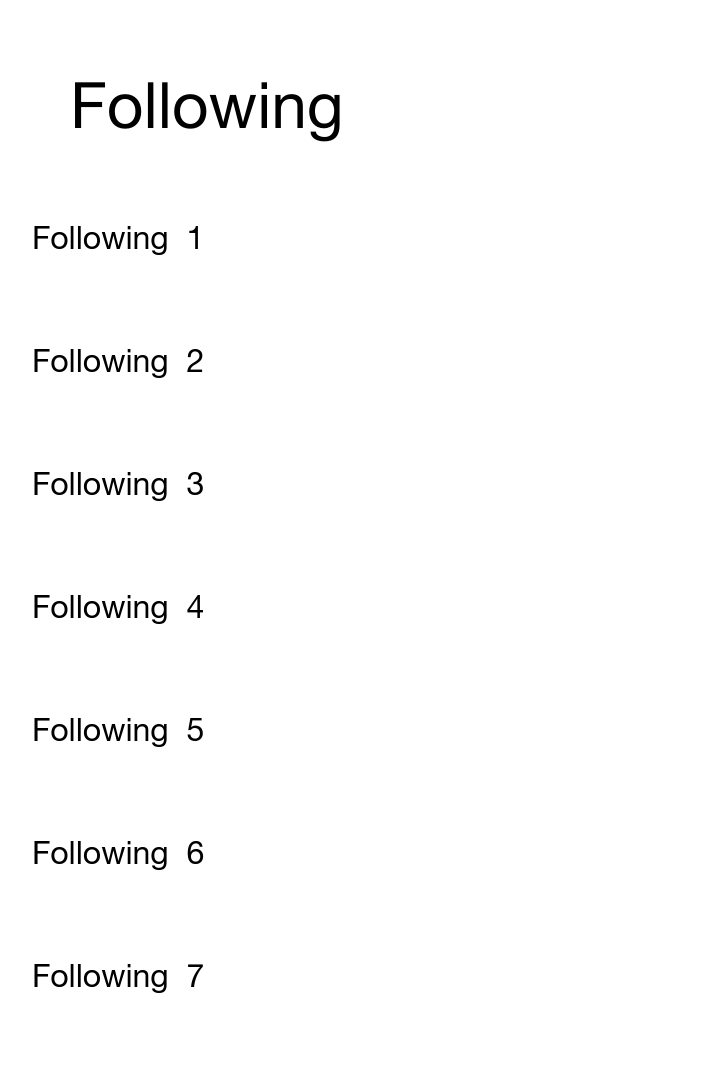
\includegraphics[scale=.20]{Following.png}}\\
\caption{Figure 6.2:  Following}
\end{center}

\newpage

\subsection{User Profile}
Here the user can see his/her profile, the people who follow him/her, the people he/she follows and his/her posts.
\begin{center}
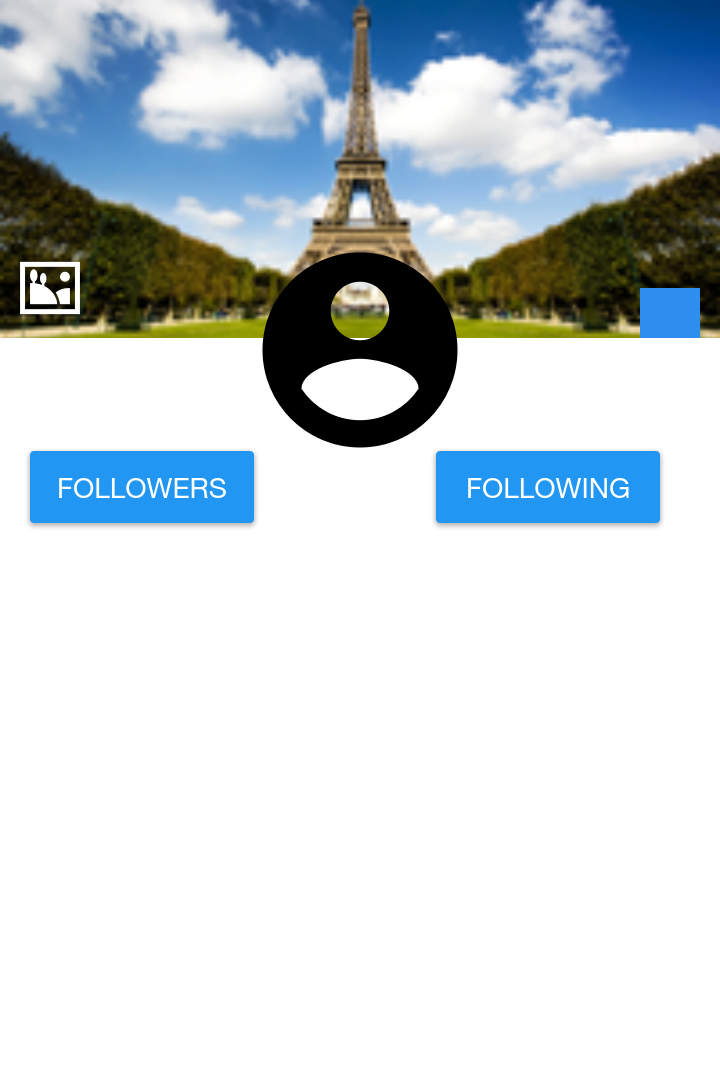
\includegraphics[scale=.40]{Profile.png}}\\
\caption{Figure 7:  User Profile}
\end{center}
\newpage

\subsection{Other User's Profile}
Here the user can see someone else's profile, his/her followers and posts and with an option to follow him/her.
\begin{center}
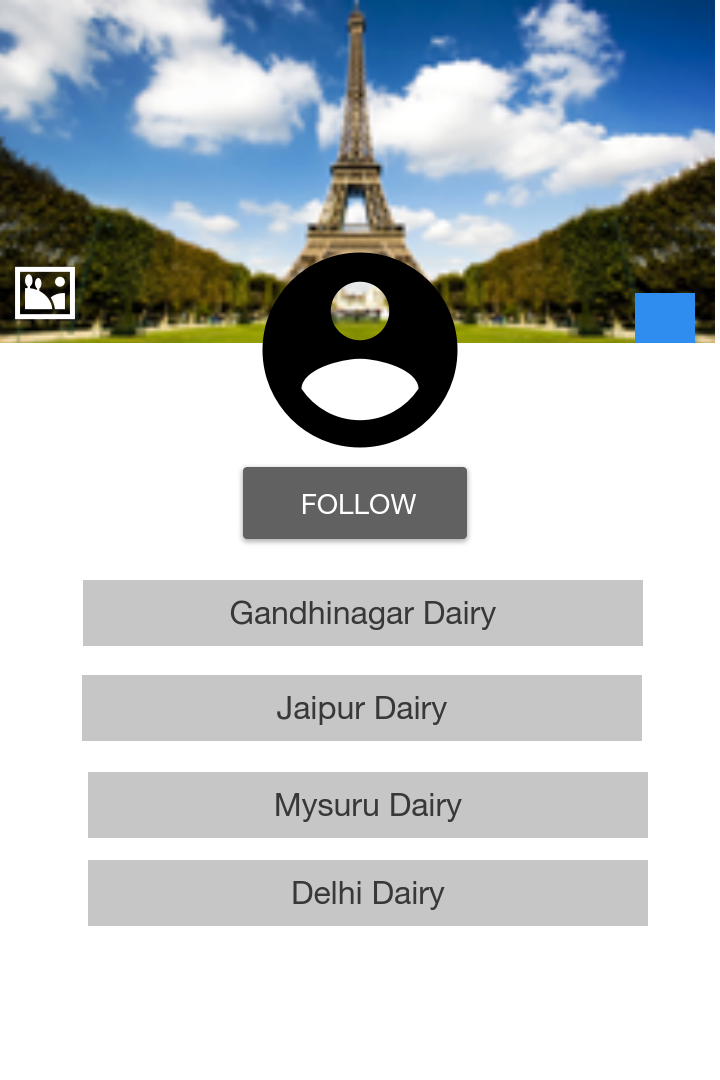
\includegraphics[scale=.40]{OtherUserProfile.png}}\\
\caption{Figure 8: Other User's Profile}
\end{center}


\end{document}
